% Тут используется класс, установленный на сервере Papeeria. На случай, если
% текст понадобится редактировать где-то в другом месте, рядом лежит файл matmex-diploma-custom.cls
% который в момент своего создания был идентичен классу, установленному на сервере.
% Для того, чтобы им воспользоваться, замените matmex-diploma на matmex-diploma-custom
% Если вы работаете исключительно в Papeeria то мы настоятельно рекомендуем пользоваться
% классом matmex-diploma, поскольку он будет автоматически обновляться по мере внесения корректив
%

% По умолчанию используется шрифт 14 размера. Если нужен 12-й шрифт, уберите опцию [14pt]
%\documentclass[14pt]{matmex-diploma}
\documentclass[14pt]{matmex-diploma-custom}
\usepackage{graphicx}

%code highlight
% \usepackage{listings}
\usepackage{listings, listings-rust}
\usepackage{lipsum}
\usepackage{xcolor}

\usepackage{tikz}
\usetikzlibrary{decorations.pathreplacing,calc,shapes,positioning}

\newcommand\tbox[1]{\tikz[overlay]\node[inner sep=2pt, draw=red, ultra thick, anchor=text, rectangle] {#1};\phantom{#1}}
 
\definecolor{codegreen}{rgb}{0,0.6,0}
\definecolor{codegray}{rgb}{0.5,0.5,0.5}
\definecolor{codepurple}{rgb}{0.58,0,0.82}
\definecolor{backcolour}{rgb}{1,1,1}
 
\lstdefinestyle{mystyle}{
    backgroundcolor=\color{backcolour},   
    commentstyle=\color{codegreen},
    keywordstyle=\color{magenta},
    numberstyle=\color{codegray},
    stringstyle=\color{codepurple},
    basicstyle=\ttfamily\small,
    breakatwhitespace=false,         
    breaklines=true,                 
    captionpos=b,                    
    keepspaces=true,                 
    numbers=left,                    
    numbersep=5pt,                  
    showspaces=false,                
    showstringspaces=false,
    showtabs=false,                  
    tabsize=2
    % xleftmargin=.2\textwidth,
    % xrightmargin=.2\textwidth
}
 
\lstset{style=mystyle}

\lstnewenvironment{code}[1][]%
{
   \noindent
   \minipage{\linewidth} 
   \vspace{0.5\baselineskip}
   \lstset{basicstyle=\ttfamily\footnotesize,frame=single,#1}}
{\endminipage}

\begin{document}
% Год, город, название университета и факультета предопределены,
% но можно и поменять.
% Если англоязычная титульная страница не нужна, то ее можно просто удалить.
\filltitle{ru}{
    chair              = {Программная инженерия\\ \vspace{5mm}Системное программирование},
    title              = {Экспериментальное исследование специализатора GPGPU-программ AnyDSL},
    % Здесь указывается тип работы. Возможные значения:
    %   coursework - Курсовая работа
    %   diploma - Диплом специалиста
    %   master - Диплом магистра
    %   bachelor - Диплом бакалавра
    type               = {bachelor},
    position           = {студента},
    group              = 471,
    author             = {Тюрин Алексей Валерьевич},
    supervisorPosition = {к.\,ф.-м.\,н., доцент},
    supervisor         = {С.\,В.~Григорьев},
    consultantPosition = {программист ООО <<Интеллиджей Лабс>>\\к.\,ф.-м.\,н.,},
    consultant         = {Д.\,А.~Березун},
    reviewerPosition   = {стажёр-исследователь\, <<ИСП\,им.\,В.\,П.~Иванникова РАН>>\\},
    reviewer           = {Е.\,Ю.\,Шарыгин},
    chairHeadPosition  = {TBD},
    chairHead          = {TBD},
%   university         = {Санкт-Петербургский Государственный Университет},
%   faculty            = {Математико-механический факультет},
%   city               = {Санкт-Петербург},
%   year               = {2013}
}
\filltitle{en}{
    chair              = {Software Engineering},
    title              = {Practical study of AnyDSL GPGPU program partial evaluator},
    author             = {Aleksey Tyurin},
    supervisorPosition = {Associate professor, Ph.\,D.},
    supervisor         = {Semyon Grigorev},
    consultantPosition = {IntelliJ Labs Co. Ltd developer\\Ph.\,D.},
    consultant         = {Daniil Berezun},
    reviewerPosition   = {Research assistant at Ivannikov Institute for System Programming of the RAS\\},
    reviewer           = {Eugene Sharygin},
    chairHeadPosition  = {TBD},
    chairHead          = {TBD},
}

\newcommand\todo[1]{{\color{violet}#1}}
\newcommand\db[1]{{\color{red}#1}}
\newcommand\question[1]{{\color{cyan}#1}}

\maketitle
\tableofcontents
% У введения нет номера главы
\chapter*{Введение}                         % Заголовок
\addcontentsline{toc}{chapter}{Введение}    % Добавляем его в оглавление
\textbf{Актуальность работы}

Статический анализ исходного кода является известной техникой  получения знаний о программе без её исполнения ~\cite{StaticCodeAnalysis3,StaticCodeAnalysis2,StaticCodeAnalysis1}. Статический анализ является неотъемлемой частью многих процессов, связанных с разработкой программного обеспечения (ПО), и может использоваться, например, для упрощения работы с кодом с помощью подсветки синтаксиса языка в программах, навигации по коду, реализации контекстных подсказок. Более того, статический анализ используется для обнаружения ошибок на ранних стадиях разработки, до запуска программы, а также для поиска различных семантических ошибок, которые не могут быть определены обычным синтаксическим анализом.  Также, статический анализ используется при решении задач трансформации исходного кода и реинжиниринге~\cite{reengANT}. Однако во многих языках программирования имеются конструкции, которые существенно затрудняют статический анализ. 

Например, широко используются динамические встроенные языки --- приложение, созданное на одном языке, генерирует программу на другом языке и передаёт её на выполнение в соответствующее окружение. Примерами могут служить динамические SQL-запросы к базам данных из приложений на Java, С++, С\#, формирование HTML-страниц в PHP-приложениях~\cite{DSQLISO,JSP,PHPmySQL}. Генерируемый код собирается из строк таким образом, чтобы в момент выполнения результирующая строка представляла собой корректную программу. Примеры использования встроенных языков представлены в листингах~\ref{lst:dsql1},~\ref{lst:JsJava} и~\ref{lst:PhPSqlHtml}. Следует отметить, что одна программа может генерировать код на нескольких языках (см. листинг~\ref{lst:PhPSqlHtml}). При этом возможно получение частей кода из разных источников (например, учитывать текстовый ввод пользователя, что часто используется для задания фильтров при конструировании SQL-запросов). Использование динамически формируемых программ  позволяет избежать дополнительных накладных расходов, присущих таким технологиям, как ORM\footnote{ORM или Object-Relational Mapping --- технология программирования, которая связывает базы данных с концепциями объектно-ориентированных языков программирования~\cite{ORM}.}, и достичь высокой производительности. Благодаря этому использование динамически генерируемых программ получило широкое распространение и применяется до сих пор. Вместе с этим, несмотря на появление новых технологий, динамическая генерация SQL-запросов активно используется и в настоящее время~\cite{DSQLInActiveUse}.

\fvset{frame=lines,framesep=5pt,fontsize=\small}\

\begin{listing}
    \begin{pyglist}[language=sql,numbers=left,numbersep=5pt]

CREATE PROCEDURE [dbo].[MyProc]  @TABLERes   VarChar(30)
AS
    EXECUTE ('INSERT INTO ' + @TABLERes + ' (sText1)' +
             ' SELECT ''Additional condition: '' + sName' +
             ' from #tt where sAction = ''1000000''')
GO
    \end{pyglist}
\caption{Код с использованием динамического SQL}
\label{lst:dsql1}
\end{listing} 
 
\fvset{frame=lines,framesep=5pt}
\begin{listing}
    \begin{pyglist}[language=java,numbers=left,numbersep=5pt]
import javax.script.*;  
public class InvokeScriptFunction {  
    public static void main(String[] args) throws Exception {  
        ScriptEngineManager manager = new ScriptEngineManager();  
        ScriptEngine engine = manager.getEngineByName("JavaScript");  
        // JavaScript code in a String  
        String script = 
            "function hello(name) { print('Hello, ' + name); }";  
        // evaluate script  
        engine.eval(script);  
        // javax.script.Invocable is an optional interface.  
        // Check whether your script engine implements or not!  
        // Note that the JavaScript engine implements
        // Invocable interface.  
        Invocable inv = (Invocable) engine;  
        // invoke the global function named "hello"  
        inv.invokeFunction("hello", "Scripting!!" );  
    }  
}
    \end{pyglist}
\caption{Вызов JavaScript из Java}
\label{lst:JsJava}
\end{listing}


\fvset{frame=lines,framesep=5pt}
\begin{listing}
    \begin{pyglist}[language=php,numbers=left,numbersep=5pt]

<?php
    // Embedded SQL
    $query = 'SELECT * FROM ' . $my_table; 
    $result = mysql_query($query);
    
    // HTML markup generation
    echo "<table>\n";
    while ($line = mysql_fetch_array($result, MYSQL_ASSOC)) {
        echo "\t<tr>\n";    
        foreach ($line as $col_value) {
            echo "\t\t<td>$col_value</td>\n";
        }
        echo "\t</tr>\n";
    }
    echo "</table>\n";
?>
    \end{pyglist}
\caption{Использование нескольких встроенных в PHP языков (MySQL, HTML)}
\label{lst:PhPSqlHtml}
\end{listing}



Динамически формируемые выражения часто конструируются с помощью таких операций, как конкатенация в циклах или условных предложениях, или в рекурсивных процедурах. Это затрудняет статический анализ и приводит к получению множества возможных значений для каждого выражения в момент выполнения. Вследствие этого фрагменты динамически формируемого кода воспринимаются компилятором исходного языка как простые строки, не подлежащие дополнительному анализу, а это, в свою очередь, приводит к высокой вероятности возникновения ошибок во время выполнения программы. В худшем случае такая ошибка не приведёт к прекращению работы приложения, что указало бы на проблемы, однако целостность данных при этом может оказаться нарушена. Более того, использование динамически формируемых выражений затрудняет не только разработку информационных систем, так и также и реинжиниринг, поскольку в последнем случае важно автоматизировать перенос системы на новые зыки и платформы, что невозможно без качественного статического анализа. Например, при наличии в коде приложения динамически формируемых SQL-запросов нельзя точно ответить на вопрос о том, с какими элементами базы данных не взаимодействует система, и удалить их. При переносе такой системы на другую СУБД необходимо гарантировать, что для всех динамически формируемых выражений значение в момент выполнения будет корректным кодом на языке новой СУБД~\cite{JSquash}. Следует отметить, что отсутствие статического анализа динамически формируемых программ не позволяет реализовывать для них стандартную функциональность интегрированных сред разработки (Integrated Development Environment, IDE) --- подсветку синтаксиса и автодополнение, рефакторинг кода и т.д. Такая функциональность значительно упрощает процесс разработки и отладки приложений и полезна не только для основного языка, но и для встроенных языков. 

Для решения всех перечисленных выше задач необходимы инструменты, проводящие статический анализ динамически формируемых программ. Такой анализ может дать существенную информацию о таких программах, поскольку редко встречается ситуация полной динамической неопределённости (например, при создании динамических программ исключительно на основе пользовательского ввода). В большинстве случаев, имея программу, генерирующую динамические вставки, с помощью статического анализа можно получить достаточно информации для решения поставленных выше задач. Решению этой проблемы и посвящена данная диссертационная работа. 


\textbf{Степень разработанности темы}

Существуют классические исследования, посвященные разработке компиляторов --- работы А.~Ахо~\cite{Dragon}, А.~Брукера~\cite{CompilerCompiler}, С.~Джонсона~\cite{yaccBook},  Б.К.Мартыненко~\cite{Martinenko1, Martinenko2}  и др.  Однако содержащиеся там алгоритмы синтаксического анализа не могут быть применены к решению задачи анализа динамически формируемых программ, поскольку предназначены для обработки входных данных, представимых в видн линейной последовательности символов, а такое представление динамически формируемых программ не всегда возможно.

Методы обобщённого синтаксического анализа, лежащие в основе данной работы, изложены в трудах таких учёных как Масару Томита (Masaru Tomita)~\cite{Tomita}, Элизабет Скотт (Elizabeth Scott) и Адриан Джонстон (Adrian Johnstone)~\cite{RNGLR,RIGLR} из университета Royal Holloway (Великобритания), Ян Рекерс (Jan Rekers, University of Amsterdam)~\cite{SPPF}, Элко Виссер (Eelco Visser)~\cite{RNGLRSyntaxerror2,RNGLRSyntaxerror3} и других.

Анализу динамически формируемых строковых выражений посвящены работы таких зарубежных учёных как Кюнг-Гу Дох (Kyung-Goo Doh)~\cite{LrAbstract1,LrAbstract2,LRAbstractParsingSema}, Ясухико Минамиде (Minamide Yasuhiko)~\cite{PHPSA}, Андерс Мёллер (Anders M{\o}ller)~\cite{JSA} и отечественных учёных А.А.~Бреслава~\cite{Alvor1,Alvor2} и других. Хорошо изучены вопросы проверки корректности динамически формируемых выражений и поиска фрагментов кода, уязвимых для SQL-инъекций~\cite{SQLInjection,Dasgupta:2009:SAF:1546683.1547548}. Однако данные работы исследуют отдельные аспекты проблемы статического анализа динамически формируемых программ, оставляя в стороне создание готовых алгоритмов (в частности, не строят структурное представление анализируемых программ). В связи с этим возникают проблемы масштабируемости данных результатов, например, создание на их основе более сложных видов статического анализа.

Так же важным является предоставление компонентов, упрощающих создание новых инструментов для решения конкретных задач. Данных подход хорошо исследован в области разработки компиляторов, где широкое распространение получили генераторы анализаторов и пакеты стандартных библиотек (работы А.~Ахо~\cite{Dragon}, А.~Брукера~\cite{CompilerCompiler}, С.~Джонсона~\cite{yaccBook} и др.). 

В работах отечественных учёных М.Д.~Шапот и Э.В.~Попова~\cite{DynamicDSQLTranslation}, а так же зарубежных учёных Антони Клеви (Anthony Cleve), Жан-Люк Эно (Jean-Luc Hainaut)~\cite{DSQLReverseEngineering}, Йост Виссер (Joost Visser)~\cite{DSQLQualityMesure} и других рассматриваются различные аспекты реинжиниринга информационных систем, использующих встроенные SQL-запросы, однако не формулируется общего метода для решения таких задач. Этот вопрос также не затрагивается в классических работах, посвященных реинжиниригу~\cite{SoftwareReeng1, reengANT, SoftwareReeng2, SoftwareReeng3}. Однако разработка такого метода является актуальной задачей.

Таким образом, актуальной является задача дальнейшего исследования статического анализа динамически формируемых строковых выражений. Кроме этого важным является решение вопросов практического применения средств анализа динамически формируемого кода: упрощение разработки инструментов анализа и создание методов их применения в реинжиниринге программного обеспечения.
\textbf{Объект исследования}

Объектом исследования являются методы, алгоритмы и программные средства обработки динамически формируемых программ, а также задача реинжиниринга информационных систем.

\textbf{Цель и задачи диссертационной работы}

\textbf{Целью} данной работы является создание комплексного подхода к статическому синтаксическому анализу динамически формируемых программ.

Достижение поставленной цели обеспечивается решением следующих \textbf{задач}.
\begin{enumerate}
    \item Разработать универсальный алгоритм синтаксического анализа динамически формируемых программ, не зависящий от целевого языка программирования и допускающий реализацию различных видов статического анализа. 
    \item Создать архитектуру инструментария для автоматизации разработки программных средств статического анализа динамически формируемых программ.
    \item Создать метод реинжиниринга динамически формируемых программ.
\end{enumerate}

\textbf{Методология и методы исследования}

Методология исследования основана на подходе к спецификации и анализу формальных языков, активно развивающемуся с 50-х годов 20-го века (см., например, работы Н. Хомского~\cite{chomskyMethod ,chomskySyntactic}). В последствии этот подход получил широкое распространение в областях, связанных с обработкой языков программирования.
Основными элементами данного подхода являются алфавит и грамматика языка, разбиение автоматической обработки языка на выполнение таких шагов как лексический, синтаксический и семантический анализ. Решаемые в связи с этим задачи связаны с поиском эффективных алгоритмов, выполняющих эти шаги. 

В работе применяется алгоритм обобщённого восходящего синтаксического анализа RNGLR~\cite{RNGLR}, созданный Элизабет Скотт (Elizabeth Scott) и Адриан Джонстон (Adrian Johnstone) из университета Royal Holloway (Великобритания). Для компактного хранения леса вывода использовалась структура данных Shared Packed Parse Forest (SPPF), которую предложил Ян Рекерс (Jan Rekers, University of Amsterdam)~\cite{SPPF}.

Доказательство завершаемости и корректности предложенного алгоритма проводилось с применением теории формальных языков, теории графов и теории сложности алгоритмов. Приближение множества значений динамически формируемого выражения строилось в виде регулярного множества, описываемого с помощью конечного автомата.


\textbf{Положения, выносимые на защиту}
\begin{enumerate}
    \item Разработан алгоритм синтаксического анализа динамически формируемых программ, позволяющий обрабатывать произвольную регулярную аппроксимацию множества значений выражения в точке выполнения, реализующий эффективное управление стеком и гарантирующий конечность представления леса вывода. Доказана завершаемость и корректность предложенного алгоритма при обработке регулярной аппроксимации, представимой в виде произвольного конечного автомата без $\varepsilon$-переходов. 
    \item Создана архитектура инструментария для разработки программных средств статического анализа динамически формируемых программ.
    \item Разработан метод анализа и обработки динамически формируемых программ в проектах по реинжинирингу информационных систем. 
\end{enumerate}

\textbf{Научная новизна работы}

Научная новизна полученных в ходе исследования результатов заключается в следующем.

\begin{enumerate}

\item Алгоритм, предложенный в диссертации, отличается от аналогов (работы Андрея Бреслава~\cite{Alvor1, Alvor2}, Кюнг-Гу Дох~\cite{LrAbstract1, LrAbstract2}, Ясухико Минамиде~\cite{PHPSA}) возможностью построения компактной структуры данных, содержащей деревья вывода для всех корректных значений выражения. Это позволяет использовать результаты работы алгоритма для проведения более сложных видов анализа. Алгоритмы, представленные в (JSA~\cite{JSA}~\cite{Alvor1, Alvor2}, PHPSA~\cite{PHPSA}) предназначены только для проверки корректности выражений, основанной на решении задачи о включении одного языка в другой. Выполнение более сложных видов анализа, трансформаций или построения леса разбора не предполагается. 

\item Новизна представленной архитектуры заключается в том, что она позволяет создать платформу для разработки целевых инструментов, решающих широкий круг задач анализа динамически формируемого кода. Существующие архитектуры готовых инструментов (JSA, PHPSA, Alvor, Varis) предназначены для решения конкретных задач для определённых языков. Решение новых задач или поддержка других языков с помощью этих инструментов затруднены ввиду ограничений, накладываемых архитектурой и возможностями используемого алгоритма анализа. 

\item Метод анализа и обработки встроенного программного кода в проектах по реинжинирингу информационных систем предложен впервые. К.В.~Ахтырченко и Т.П.~Сорокваша отмечают~\cite{SoftwareReengMethods}, что существующие работы в области реинжиниринга программного обеспечения либо содержат высокоуровневые решения, не касающиеся деталей, важных при решении прикладных задач (например, работы К. Вагнера~\cite{SoftwareReeng3}, Х. Миллера~\cite{SoftwareReeng2}), либо являются набором подходов к решению конкретных задач (например, работы~\cite{SoftwareReeng1, reengANT, boulychev}). При этом, встроенный программный код часто не учитывается. С другой стороны, работы М.Д.~Шапот и Э.В.~Попова~\cite{DynamicDSQLTranslation}, С.Л.~Трошина~\cite{reengANT}, А.~Клеви~\cite{DSQLReverseEngineering}  посвящены решению конкретных задач обработки встроенного программного кода в контексте реинжиниринга информационных систем, но не предлагают обобщённого и масштабируемого метода.

\end{enumerate}


\textbf{Теоретическая и практическая значимость работы}

Теоретическая значимость диссертационного исследования заключается в разработке формального алгоритма синтаксического анализа динамически формируемого кода, решающего задачу построения конечного представления леса вывода, не решенную полностью ранее, а также в формальном доказательстве завершаемости и корректности разработанного алгоритма. 

На основе полученных в работе научных результатов был разработан инструментарий (Software Development Kit, SDK), предназначенный для создания средств статического анализа динамически формируемых программ. 
С использованием разработанного инструментария было реализовано расширение к инструменту ReSharper (ООО ``ИнтеллиДжей Лабс'', Россия), предоставляющее поддержку встроенного T-SQL в проектах на языке программирования C\# в среде разработки Microsoft Visual Studio. Так же было выполнено внедрение результатов работы в промышленный проект по переносу хранимого SQL-кода с MS-SQL Server 2005 на Oraclе 11gR2 (ЗАО ``Ланит-Терком'', Россия). 

\textbf{Степень достоверности и апробация результатов}

Достоверность и обоснованность результатов исследования опирается на использование формальных методов исследуемой области, проведенные доказательства, рассуждения и эксперименты.

Основные результаты работы были доложены на ряде научных конференций: SECR-2012, SECR-2013, SECR-2014, TMPA-2014, Parsing@SLE-2013, Рабочий семинар ``Наукоемкое программное обеспечение'' при конференции PSI-2014. Доклад на SECR-2014 награждён премией Бертрана Мейера за лучшую исследовательскую работу в области программной инженерии. Дополнительной апробацией является то, что разработка инструментальных средств на основе предложенного алгоритма была поддержана Фондом содействия развитию малых форм предприятий в технической сфере (программа УМНИК~\cite{UMNIC}, проекты \textnumero~162ГУ1/2013 и \textnumero~5609ГУ1/2014).

\textbf{Публикации по теме диссертации}

Все результаты диссертации изложены в 7 научных работах, из которых 3~\cite{YCArticle,SELforIDEru,AbstractGLL}, содержащие основные результаты, опубликованы в журналах из ‘’Перечня российских рецензируемых научных журналов, в которых должны быть опубликованы основные научные результаты диссертаций на соискание ученых степеней доктора и кандидата наук’’, рекомендовано ВАК. 
1 работа~\cite{GLRAbsPars} индексируются Scopus. В работах, написанных в соавторстве, вклад автора определяется следующим образом.  В~\cite{Syrcose} С. Григорьеву принадлежит реализация ядра платформы YaccConstructor. В~\cite{SELforIDEru, AbstractGLL} и~\cite{SELforIDE} С. Григорьеву принадлежит постановка задачи, формулирование требований к разрабатываемым инструментальным средствам, работа над текстом. 
В~\cite{GLRAbsPars} автору принадлежит идея, описание и реализация анализа встроенных языков на основе RNGLR алгоритма.  В~\cite{YCArticle} С. Григорьеву принадлежит реализация инструментальных средств, проведение экспериментов, работа над текстом. В работе~\cite{RelaxedARNGLR} автору принадлежит алгоритм синтаксического анализа динамически формируемого кода.


\textbf{Структура работы}

Диссертация состоит из введения, шести глав, заключения и построена следующим образом. В первой главе приводится обзор области исследования. Рассматриваются подходы к анализу динамически формируемых строковых выражений и соответствующие инструменты. Описывается алгоритм обобщённого восходящего синтаксического анализа RNGLR, взятый за основу в диссертационной работе. Также описываются проекты YaccConstructor и ReSharper SDK, использованные для реализации предложенного в работе инструментария. Во второй главе формализуется основная задача исследования и излагается решающий её алгоритм синтаксического анализа регулярных множеств. Приводится доказательство завершаемости и корректности представленного алгоритма, приводятся примеры. В третьей главе описывается инструментальный пакет YC.SEL.SDK, разработанного на основе алгоритма, описанного во второй главе и предназначеного для разработки инструментов анализа динамически формируемых программ. Описывается архитектура компонентов и особенности их реализации. Также описывается YC.SEL.SDK.ReSharper --- ``обёртка'' для YC.SEL.SDK, позволяющая создавать расширения к ReSharper для поддержки встроенных языков. В четвёртой главе описывается метод реинжиниринга встроенного программного кода.  В пятой главе приводятся результаты экспериментального исследования разработанного алгоритма и инструмента YC.SEL.SDK. Шестая глава содержит результаты сравнения и соотнесения полученных результатов с  существующими аналогами.

\textbf{Благодарности}

А.Н.Терехову, работкникам и администрации компании ЗАО ``Ланит-Терком'' за создания условий для изучения данной темы (организация проектов по реинжинирингу). Я.А.Кириленко за погружение в тему исследования и руководство на начальных этапах. Д.Ю.Булычеву за помощь в уточнении постановки задачи исследования и в написании статей. Студентам и аспирантам кафедры системного программирования Дмитрию Авдюхину, Анастасии Рагозиной, Екатерине Вербицкой, Марине Полубеловой, Иванову Андрею за помощь в реализации предложенных идей и проведение экспериментов. Отдельную благодарность  хочется выразить компании ООО ``ИнтеллиДжей Лабс'' и Андрею Иванову за поддержку исследований. Также хочется поблагодарить А.К.Петренко и В.М.Ицыксона, а также сотрудников ИСП РАН за ценные вопросы и комментарии к работе, позволившие уточнить ряд формулировок и улучшить изложение результатов. 

\section*{Problem statement}\label{ps}
The aim of the work is the practical evaluation of whether any performance enhancement could be brought %by partial evaluation technique
by partially evaluating memory accesses through the utilization of AnyDSL framework, compared to CUDA implementations, considering GPU microarchitecture details that affect the result. In order to achieve the aim, the following objectives have been set.
\begin{itemize}
    \item Implement experimental scenarios in both AnyDSL and CUDA.
    \item Collect relevant datasets for the evaluation to be more practical.
    \item Perform the evaluation and analyze the results.
\end{itemize}

More specifically, the work performs the evaluation on string matching and convolutional filtering scenarios, providing some relevant CUDA assembly examples to ground the effects being observed.

% Firstly, the hypothesis of whether GPU-based string pattern matching program performance speed up could be achieved via partially evaluating memory accesses, should have been verified. A modern GPU has different types of memory, varying by access latency. In order to achieve maximal performance every type of memory should be utilized carefully, satisfying alignment and access patterns requirements. Moreover, several cache levels are extensively used to mitigate the latency, and, to some extent, caches could keep up the performance of an application, even if a proper access pattern is hard to achieve. There is a partial evaluator, being developed as part of AnyDSL framework~\cite{LeiBa}, with the support for generation of specialized Nvidia CUDA C code. It has been utilized to verify the hypothesis.   

% Next, the bottlenecks that arise during string pattern matching program specialization should be identified. Particular program transformations could potentially hurt further parallelization or simply not achieve expected effects. Thus, string pattern matching algorithms specialization should be examined using available partial evaluators.

% Then the partial evaluator should be implemented considering the identified bottlenecks either from scratch or as an extension for available ones.

% Finally, the obtained partial evaluator efficiency should be evaluated through performance comparison between specialized programs and manually fine-tuned ones.   
\section{Related work \& background}
This section gives the necessary insights about a typical GPU architecture, performance-related considerations, and differences between compute capabilities from CUDA perspective, as well as known approaches for memory optimizations, while also providing the insights about partial evaluation and its known practical applications.
\subsection{Nvidia CUDA}
Modern GPUs are highly parallel computational devices equipped with a very high-bandwidth memory, designed to speed up general-purpose computations. CUDA defines a specific programming model\footnote{\url{https://docs.nvidia.com/pdf/CUDA_C_Programming_Guide.pdf} \\ (last accessed date: 30.05.2020)} and architecture for NVIDIA GPUs. These details are provided considering Nvidia Tesla T4 GPU.
\paragraph*{Hardware architecture}
Nvidia Tesla T4\footnote{\url{https://www.nvidia.com/content/dam/en-zz/Solutions/design-visualization/technologies/turing-architecture/NVIDIA-Turing-Architecture-Whitepaper.pdf} (last accessed date: 30.05.2020)} GPU is of Turing architecture and constitutes of five Graphics Processing Clusters (i.e. self-contained GPUs), each including four Texture Processing Clusters that incorporates two Streaming Multiprocessors (SM) each. Each SM is built up of four processing blocks, each including a warp\footnote{A batch of 32 CUDA threads} scheduler, dispatch unit, and units for a memory fetch, integer, and floating-point operations, latter being called CUDA-cores. The GPU includes 2560 of such cores. Further, Tesla is supplied with 16GB GDDR6 memory that supports throughput up to 320GB/s. Unlike previous architectures it incorporates shared memory in L1 cache, increasing the bandwidth up to 2x, and adds an independent integer datapath, enabling concurrent execution of integer and floating-point operations. Finally, Tensor Cores has been introduced, being specialized execution units specifically for performing the tensor/matrix operations.

\paragraph*{Programing model}
CUDA implies Single Instruction Multiple Threads architecture, where each instruction is concurrently executed by multiple threads, that are combined in blocks, that populates a grid. Threads in a block are split into warps, which are distributed between warp schedulers on a single SM, such schedulers assign per-thread instructions to the available computation units. Hence, in general, threads in a warp should execute the same instruction to achieve the best performance, in case of different instructions, caused e.g. by an if-statement, the execution is serialized, this is called a \emph{thread-divergence}. A piece of a program that is intended to be executed on a GPU is called a device kernel and usually is implemented in CUDA C, where grid and block sizes also could be specified.

\begin{figure}[t]
    \centering
    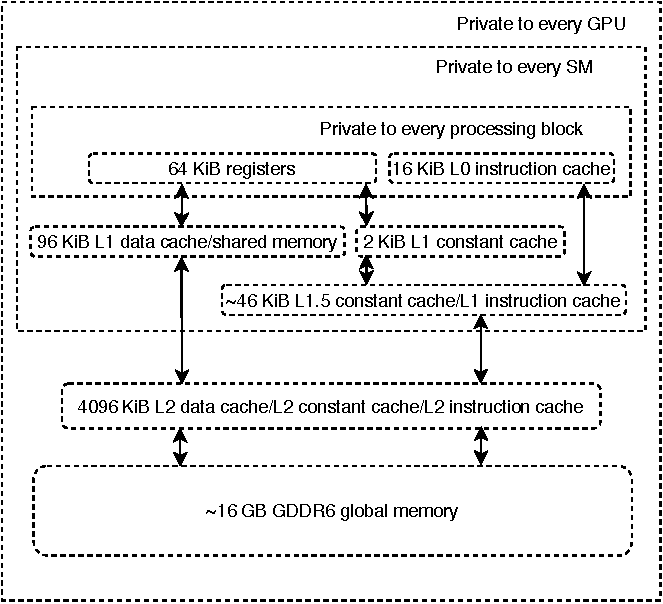
\includegraphics{figures/TeslaT4Mem.pdf}
    \caption{Nvidia Tesla T4 memory hierarchy~\cite{TeslaT4Bench}}
    \label{fig:t4_mem}
\end{figure}

\paragraph*{Memory hierarchy}
Any GPU incorporates several memory types, that serve different purposes and differ in access latency, size, and bandwidth.
The memory architecture of Tesla T4 is depicted in \ref{fig:t4_mem}.

\emph{Global memory} is the main resource to transfer data between host and device. It is the largest and the slowest memory space, cacheable in L1 and L2 caches, that have 32 B and 64 B lines respectively.
Global memory loads and stores by threads of a warp are served by the device with 32 B transactions\footnote{\url{https://docs.nvidia.com/cuda/pdf/CUDA\_C\_Best\_Practices\_Guide.pdf} (last accessed date: 30.05.2020)}.
Basically, concurrent accesses of the threads in a warp will coalesce into a number of such transactions necessary to service all the threads in the warp.
So in order to keep the number of such transactions to a minimum, threads in a warp should access adjacent segments of memory, aligned with the transaction size, avoiding strided accesses.
Such a requirement could not always be satisfied in practice, thus GPU resources being used not to its maximum. This memory space is accessible and allocated from the host, and visible to all the threads in a grid. 

\emph{Shared memory} is on-chip memory (hence it has lower latency and higher bandwidth than global memory) used to optimize frequent accesses to the same elements in global memory.
It is fast as long as bank conflicts do not occur.
The whole shared memory space is divided into 32 banks --- 4 B memory elements, with successive 4 B words belonging to successive banks. 
Any bank has a bandwidth of 4 B per clock cycle.
Therefore, any memory load or store of $n$ addresses, belonging to n distinct memory banks
could be serviced simultaneously with the bandwidth of $n$ times the bandwidth of a single bank.
However, accesses to memory addresses from the same bank are serialized, decreasing the effective bandwidth in a magnitude of the number of conflict-free accesses. When multiple threads of a warp access the same shared memory, a broadcast occurs. Several such broadcasts could coalesce into a single multicast. This memory space has a visibility scope of a single thread block and is not accessible from the host.

\emph{Constant memory} is a cacheable off-chip memory, that is read-only from the device. It is a 64 KB part of global memory, that has a specific path for caching. As a result, on a cache miss, a constant memory read costs one memory read from global memory; otherwise, it is as fast as register access. When the threads in a warp access different constant memory addresses, these accesses are serialized.  Thus the constant cache is best when the threads in warp access the same or very few distinct addresses, in the first case the access is broadcasted, and the latency is the same as registers one.

\emph{Register memory} is on-chip memory, consuming zero extra clock cycles per instruction, as long as there is no register read-after-write dependencies and bank conflicts. Is has a scope of a single thread and is the fastest memory type available.


\subsection{Memory optimizations}
Given such a sophisticated memory hierarchy that should be managed by a programmer, memory optimizations are in a great interest. Only automatic memory optimizations would be considered, avoiding the guidelines about how to rearrange existing access patterns and speed-up the transferring between host and device.

In cases when abundant data parallelism is hard to achieve, e.g. when utilizing concurrent data structures and related synchronization primitives that arbitrate the accesses, dynamic memory allocation, i.e. per-thread allocation inside the device code, for such data structures becomes a bottleneck, hurting the throughput. In~\cite{NvidiaAllocator} a novel approach for dynamic memory allocation is proposed. It is based on shared data structures, supporting fine-grained mutual exclusion regions, cooperative synchronization primitives allowing to allocate memory concurrently between the threads, and a policy of execution delegation. The proposed allocator has a much higher allocation throughput compared to the one, deployed with CUDA.

Since the register memory is bounded in size, excessive registers\footnote{When the compiler needs more registers, than available on SM.} could be spilled into the global memory, introducing higher latency. 
Contrary to the default CUDA compiler approach, that handles excessive registers via re-materialization\footnote{Recomputation of a value instead of loading and storing.
It produces the code with lower efficiency, however with lower register usage as well.} as long as possible before spilling, an approach from~\cite{RegisterSpilling} advocates the usage of underutilized shared memory to spill the excessive registers.
The approach is implemented as an extra binary translation pass over CUDA assembly.
Under certain conditions, such optimization is worse than CUDA default approach, thus the authors also provide a compile-time performance gain estimator, based on collected either explicit or implicit\footnote{Some stalls are labeled by the compiler, others are deduced, based e.g. on latencies for the memory type being accessed by the instruction.} instruction stalls, to compare the default code produced by the compiler and an optimized one, to decide which one is better.
On average, this technique achieves 10\% better performance on the selected benchmarks.

Another work is focused at the automatic allocation of shared memory to reduce the number of global memory transactions~\cite{AutomaticSharedMem} for automatically C-to-CUDA generated programs.
Authors propose a performance model, designed to choose the best configuration for shared memory allocation, considering estimated execution time, memory metrics, and the number of reduced global memory transactions.
Once the best configuration is found, it is applied
to the original C code by adding specific OpenACC\footnote{A set of directives for heterogeneous code parallelization} pragmas.

To tackle the problem of the lack of available GPU memory, a domain-oriented memory pooling and swapping is proposed in~\cite{zhang2019efficient}. Variables not in use are swapped to host and swapped back before any access, while variables that have non-overlapping lifetime could be allocated to the same memory space by the heuristic-driven memory pool. The heuristic is based on the iterative nature of the deep learning training algorithms to derive the lifetime and read/write order of all variables.

%тут бы переход какой-то к след подсекции
Despite such a variety of different memory optimization approaches, none of the presented works exploits possible static nature of device kernel parameters in any way. Thus, the application of partial evaluation technique to GPU kernels could provide another optimization approach, oriented at static data management.

\subsection{Partial evaluation}\label{PEsurvey}
%написать про partial evaluation с примером
\emph{Partial evaluation} is a program transformation and optimization technique, also known as program \emph{specialization}, first formulated in~\cite{Kleene1952-KLEITM}.
A partial evaluator is an algorithm, that takes a program and some of its known inputs called \emph{static} and produces another residual program, one yielding the same result given the remaining \emph{dynamic} inputs as the original program would have produced given all the inputs at once as illustrated in commutative diagram~\ref{fig:mix}.
A partial evaluator performs a mixture of code generation and execution: it reduces those parts of program \textbf{p}, depending on \textbf{in1}, and generates code for calculations for yet unavailable \textbf{in2}.
Generally, it performs symbolic computations, unfolding function calls, and replacement of function calls to their specialized versions.
For example, a partial evaluator for the program in listing~\ref{fig:pow} reduces the number of static conditional statements driven by static parameter. 

\begin{figure}
    \centering
    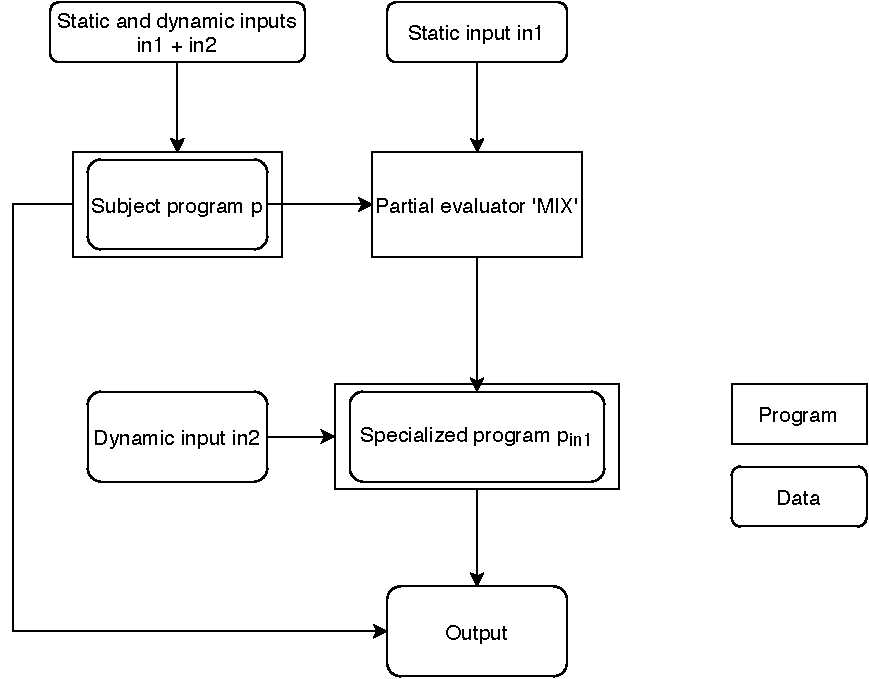
\includegraphics{figures/MixCommutativity.pdf}
    \caption{Partial evaluation pipeline}
    \label{fig:mix}
\end{figure}

The key idea is that a specialized program requires fewer computations (through moving them to compile or specialization time), and thus is intended to be more effective. A notable feature of specialization is the ability to generate a compiled program, once given an interpreter and a source program, also known as the first Futamura projection~\cite{Futamura1999}.
And while many practical applications benefit from partial evaluation through reducing the interpretation overhead (either by generating a compiler or exploiting interpretative nature of a program), there are scenarios, when a program takes more than one input, and one of the inputs varies more slowly than the others, thus specialization with respect to less-variable input could produce a more effective program.
Significant speed-up results were reported for pattern recognition, ray tracing, database querying, and scientific computing~\cite{Jones1993}.

\begin{code}[language=C,label=fig:pow,caption=Pow function partial evaluation example]
int pow(int x,int n){
    if (n == 0) return 1;
    else if (n \% 2 == 0) { 
        return pow2(f(x,n/2));
    }
    else return x * f(x,n-1);
}
//partially evaluating pow(x,5) would yield:
int pow(int x){
    return x * pow2(pow2(x));
}
\end{code}

In~\cite{JavaPe} an annotation-driven partial evaluator for Java programming language is introduced.
The goal is to specialize framework configurations and quite expensive reflection calls, which are widespread in object-oriented systems. The replacement of reflective method calls with partially evaluated ordinary calls allows to speed-up a dynamic pricing system by a power of six.

In~\cite{SuperVm} an approach for automatic virtual machine construction is proposed, which allows new languages to be implemented through the specification of abstract syntax tree interpreter. Partial evaluation is used to compile hot and stable parts of the already specialized\footnote{Supplied with runtime information such as types.} interpreter.

Another usage of partial evaluation as a means for compilation has been described in~\cite{LLVM-mix}. The PostgreSQL query interpreter, compiled at first to LLVM IR, which the designed partial evaluator works with, has been specialized in runtime with respect to the query, i.e. the query is compiled. The approach results in rather significant performance improvement, requires fewer efforts compared to just-in-time compiler development and is fully automatic.


Despite such a broad variety of partial evaluation- related research, at the moment of writing, there is a lack of research combining GPGPU and partial evaluation.
In~\cite{JitGPUPE} the approach from~\cite{SuperVm} was adopted to compile code from \emph{R} language to \emph{OpenCL}, to make it possible to write GPU-accelerated applications with dynamic interpreted languages, popular in big data, ignoring third-party libraries and relatively low-level programming languages for GPU. A metaprogramming system for writing shaders is presented in~\cite{GPUsh}, which supports partial evaluation via currying. However, the system is rather outdated and has no relation to modern GPGPU programming. Furthermore, there are no works dedicated to what benefits partial evaluation could provide once applied directly to GPU program, or whether it could provide any at all.

\begin{code}[language=Java,label=fig:kernel,caption=A typical GPGPU kernel]
handleData (filterParams, data)
{
  res = new List()
  for d in data
     for e in filterParams
        if d % e == 0
        then res.Add(d)
  return res
}
\end{code}


%$\llbracket \llbracket mix \rrbracket %[handleData,[2;3]]\rrbracket$
\begin{code}[language = Java, label = fig:kernel_mix,caption={ A typical GPGPU kernel specialization with respect to {[2;3]}}]
handleData (data)
{
  res = new List()
  for d in data
    if d % 2 == 0 ||
       d % 3 == 0
    then res.Add(d)
  return res
}
\end{code}

However, in practice, it appears that many GPGPU scenarios could have static parameters in a sense, theoretically appropriate for specialization.
A typical GPGPU kernel is depicted in listing~\ref{fig:kernel}.
It often represents some kind of a filter, that is applied to different pieces of the data in parallel by a huge number of threads.
The execution time primarily depends on the size of the data, which often exceeds the available memory of GPU, therefore the device kernel is run multiple times on different chunks of the data, resulting in significant execution time.
Hence, the filter varies less frequently than the data and could be considered as a static input and subjected to specialization.
However, the filter becomes known at runtime, before the kernel actually runs, thus the specialization should be performed at runtime.
The overhead of the partial evaluation could be hidden by the gained speed-up across the long run of the kernel.
Moreover, since one filter could be applied to different data pieces, the specialized version could be cached and reused instead of specializing again. The effect of specialization could be seen in listing~\ref{fig:kernel_mix}.
The inner cycle with accesses to the memory space of the filter has been reduced with the filter parameters being placed directly into the instructions.
Since memory access operations have been proven to be the most expensive, such a replacement could provide a benefit of accessing the filter from the registers, which is the fastest memory type, rather than from any other memory space.
Furthermore, a partial evaluator could be able to reduce those parts of the kernel, that depend on static filter parameters made available.

\subsection{AnyDSL framework}
To the date of writing, there is no partial evaluator known that works directly with CUDA C or any of CUDA intermediate representations.
As mentioned, the partial evaluator from~\cite{LLVM-mix} works with LLVM IR, and CUDA has an appropriate LLVM frontend, however, the partial evaluator leverages special attributes in IR, that conflicts with the ones of CUDA itself during LLVM JIT compilation.
AnyDSL~\cite{LeiBa} is a framework for the development of domain-specific libraries that could utilize different backends, including the one of CUDA.
The framework includes a partial evaluator that works with a specific intermediate representation, supporting CUDA C code generation.
The framework requires the programs to be developed in a special DSL named \emph{Impala}, which resembles C language with functions being the first- class objects.
Since the DSL is very CUDA C alike, the framework has been chosen as a means for partial evaluation of GPU programs.

The impala compiler translates the code into a functional graph-based intermediate representation similar to typed lambda calculus with continuations. Such a representation allows Impala to achieve near C performance, despite higher-order functions support~\cite{Thorin}.
Partial evaluation is performed on this level, while the representation could target different hardware architectures utilizing LLVM and compiler intrinsics.
An example of such an intrinsic is given in listing~\ref{impala_cuda}.
The whole function would be first converted into the intermediate representation, with the parts of the function labeled with \lstinline{@} partially evaluated, then the device-independent parts of the code would be translated into LLVM and device code would be translated into device-specific code, e.g. the code between lines 4-8 would be translated into CUDA C, which then would be included in LLVM code with a call to an external function that loads and executes the generated device code, e.g. the external function for mentioned lines would call NVIDIA CUDA compiler in runtime and launch the compiled kernel.

\begin{code}[language=Rust, label = impala_cuda, caption=Impala GPU-accelerated loop]
fn iterate(fld: Field , @body: fn(int, int) -> ()) -> () {
    let grid = (fld.cols , fld.rows , 1);
    let block = (128 , 1, 1);
    cuda(grid , block , || {
        let x = tid_x() + blockDim_x() * blockId_x();
        let y = tid_y() + blockDim_y () * blockId_y ();
        body(x, y);
    });
}
\end{code}

The authors of the framework evaluated the effectiveness of partial evaluation targeting different backends, including CUDA~\cite{LeiBa,OnlinePe}. The results show similar performance with hand-tuned third-party implementations. However, the authors focused on compile-time partial evaluation of kernels and have not provided any GPU-specific details that affect the success of the result as well as what particular optimization a partial evaluator performs with the device code. In contrast, this work is aimed at revealing GPU architecture details that affect the success of partial evaluation, focused at runtime partial evaluation and selects different experimental scenarios.


%%% Добавление поясняющих записей (notes) к презентации %%%
\makeatletter
\@ifundefined{c@presnotes}{
    \newcounter{presnotes}
    \setcounter{presnotes}{0}       % 0 --- выкл;
                                    % 1 --- вкл, записи на отдельном слайде;
                                    % 2 --- вкл, записи на основном слайде;
}{}
\makeatother

%%% Положение поясняющих записей (notes) при значении presnotes=2 %%%
\newcommand{\presposition}{left}  % возможные значения: left, right, top, bottom

%%% Добавление логотипа из файла images/logo на первом слайде %%%
\makeatletter
\@ifundefined{c@logotitle}{
    \newcounter{logotitle}
    \setcounter{logotitle}{1}       % 0 --- выкл;
                                    % 1 --- вкл
}{}
\makeatother

%%% Добавление логотипа из файла images/logo на слайдах (кроме первого и последнего) %%%
\makeatletter
\@ifundefined{c@logoother}{
    \newcounter{logoother}
    \setcounter{logoother}{0}       % 0 --- выкл;
                                    % 1 --- вкл
}{}
\makeatother

\section{Evaluation}

We evaluate the implemented algorithm on both regular and context-free path queries in order to demonstrate applicability of the proposed solution.
Namely, goals of the evaluation are following.
\begin{enumerate}
	\item Investigate the practical applicability of RPQ evaluation by the proposed algorithm.
	\item Compare Azimov's algorithm for reachability CFPQ and the proposed algorithm.
	\item Investigate the practical applicability of paths extraction algorithm for both regular and context-free queries.
\end{enumerate}

For evaluation, we use a PC with Ubuntu 18.04 installed.
It has Intel core i7-6700 CPU, 3.4GHz, and DDR4 64Gb RAM.
As far as we evaluate only algorithm execution time, we store each graph fully in RAM as its adjacency matrix in sparse format.
Note, that graph loading time is not included in the result time of evaluation.	

\subsection{RPQ Evaluation}

In oder to investigate applicability of the proposed algorithm for RPQ over real-world graphs we collect a set of real-world and synthetic graphs and evaluate queries generated by using the most popular templates for RPQs.

\subsubsection{Dataset}

Brief description of collected graphs are presented in Table~\ref{tbl:graphs_for_rpq}.
Namely, the dataset consists of several parts.
The first one is a set of LUBM graphs\footnote{Lehigh University Benchmark (LUBM) web page: \url{http://swat.cse.lehigh.edu/projects/lubm/}. Access date: 07.07.2020.}~\cite{10.1016/j.websem.2005.06.005} with a different number of vertices.
The second one is a graphs from Uniprot database\footnote{Universal Protein Resource (UniProt) web page: \url{https://www.uniprot.org/}. All files used for evaluation can be downloaded here: \url{ftp://ftp.uniprot.org/pub/databases/uniprot/current_release/rdf/}. Access date: 07.07.2020.}: \textit{proteomes}, \textit{taxonomy} and \textit{uniprotkb}.
The last part is a RDF files \textit{mappingbased\_properties} from DBpedia\footnote{DBpedia project web site: \url{https://wiki.dbpedia.org/}. Access date: 07.07.2020.} and \textit{geospecies}\footnote{The Geospecies RDF: \url{https://old.datahub.io/dataset/geospecies}. Access date: 07.07.2020.}.
These graphs represent data from different areas and they are frequently used for graph querying algorithms evaluation.

\begin{table}
{
\rowcolors{2}{black!2}{black!10}
\begin{tabular}{|l|c|c|}
\hline
Graph & \#V & \#E \\
\hline
\hline 
LUBM1k  & 120 926 & 484 646 \\
LUBM3.5k  & 358 434 & 144 9711 \\
LUBM5.9k  & 596 760 & 2 416 513 \\
LUBM1M   & 1 188 340 & 4 820 728 \\
LUBM1.7M & 1 780 956 & 7 228 358 \\
LUBM2.3M & 2 308 385 & 9 369 511 \\
\hline
Uniprotkb & 6 442 630 & 24 465 430 \\
Proteomes & 4 834 262 & 12 366 973 \\
Taxonomy & 5 728 398 & 14 922 125 \\
\hline
Geospecies & 450 609 & 2 201 532 \\
Mappingbased\_properties & 8 332 233 & 25 346 359 \\
\hline
\end{tabular}
}
\caption{Graphs for RPQ evaluation}
\label{tbl:graphs_for_rpq}
\end{table}


Queries for evaluation was generated by using templates of the most popular RPQs which are collected from~
\cite{Pacaci2020RegularPQ} (Table 2) and~\cite{Wang2019} (some of complex queries from Table 5), and are presented in table~\ref{tbl:queries_templates}.
We generate 10 queries for each template and each graph using the most frequent relations from the given graph randomly\footnote{Used generator is available as part of CFPQ\_data project: \url{https://github.com/JetBrains-Research/CFPQ_Data/blob/master/tools/gen_RPQ/gen.py}. Access data: 07.07.2020.}. 
For all LUBM graphs common set of queries was generated in order to investigate scalability of the proposed algorithm.

\begin{table}
{\small
\renewcommand{\arraystretch}{1.25}
\rowcolors{2}{black!2}{black!10}
\begin{tabular}{|c|c||c|c|}
\hline

Name & Query & Name & Query \\
\hline
\hline 
$Q_1$   & $a^*$                               & $Q_9^5$    & $(a \mid b \mid c \mid d \mid e)^+$                     \\
$Q_2$   & $a\cdot b^*$                        & $Q_{10}^2$ & $(a \mid b) \cdot c^*$                                  \\
$Q_3$   & $a \cdot b^* \cdot c^*$             & $Q_{10}^3$ & $(a \mid b \mid c)  \cdot d^*$                          \\
$Q_4^2$ & $(a \mid b)^*$                      & $Q_{10}^4$ & $(a \mid b \mid c \mid d)  \cdot e^*$                   \\
$Q_4^3$ & $(a \mid b \mid c)^*$               & $Q_{10}^5$ & $(a \mid b \mid c \mid d \mid e)  \cdot f^*$            \\
$Q_4^4$ & $(a \mid b \mid c \mid d)^*$        & $Q_{10}^2$ & $a \cdot b$                                             \\
$Q_4^5$ & $(a \mid b \mid c \mid d \mid e)^*$ & $Q_{11}^3$ & $a \cdot b \cdot c$                                     \\
$Q_5$   & $a \cdot b^* \cdot c$               & $Q_{11}^4$ & $a \cdot b \cdot c \cdot d$                             \\
$Q_6$   & $a^* \cdot b^*$                     & $Q_{11}^5$ & $a \cdot b \cdot c \cdot d \cdot f$                     \\
$Q_7$   & $a \cdot b \cdot c^*$               & $Q_{12}$   & $(a \cdot b)^+ \mid  (c \cdot d)^+$                     \\
$Q_8$   & $a? \cdot b^*$                      & $Q_{13}$   & $(a \cdot(b \cdot c)^*)^+ \mid  (d \cdot f)^+$          \\
$Q_9^2$ & $(a \mid b)^+$                      & $Q_{14}$   & $(a \cdot b \cdot (c \cdot d)^*)^+  \cdot (e \mid f)^*$ \\
$Q_9^3$ & $(a \mid b \mid c)^+$               & $Q_{15}$   & $(a \mid b)^+ \cdot (c \mid d)^+$                       \\
$Q_9^4$ & $(a \mid b \mid c \mid d)^+$        & $Q_{16}$   & $a \cdot b \cdot (c \mid d \mid e)$                     \\
\hline
\end{tabular}
}
\caption{Queries' templates for RPQ evaluation}
\label{tbl:queries_templates}
\end{table}


\subsubsection{Results}

For reachability index creation average time of 5 runs is presented.

Reachability index creation time for each query for LUBM graphs set is presented in figure~\ref{fig:lubm_all_qs}.
We can observe linear !!!! dependency of evaluation time on graph size.
Also we can see, that query evaluation time depends on query: there are queries which evaluate less then 1 second even for biggest graph ($Q_2$, $Q_5$, $Q_{11}^2$, $Q_{11}^3$), while worst time is 6.26 seconds ($Q_{14}$).
Anyway, we can argue that in this case our algorithm demonstrates reasonable time to be applied for real-world data analysis, because it is comparable with recent results on the same problem for LUBM querying by using distributed system over 10 nodes~\cite{Wang2019}, while we use only one node. 
Note, that accurate comparison of different approaches is a huge interesting work for the future.

\begin{figure}
   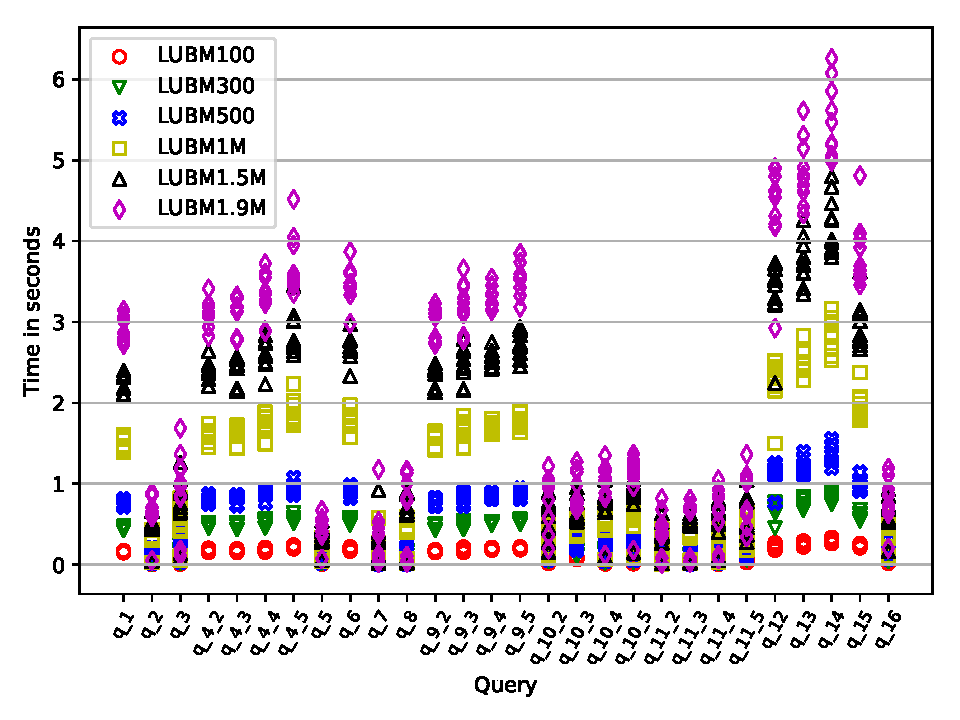
\includegraphics[width=0.48\textwidth]{data/LUBM_all.pdf}
   \caption{Reachability index creation time for LUBM graphs}
   \label{fig:lubm_all_qs}
\end{figure}

Reachability index creation time for each query for for real-world graphs is presented in figure~\ref{fig:other_all_qs}.
We can see that query evaluation time depends on graph inner structure. 
First of all, in some cases handling of small graph requires more time, then handling bigger graph.
For example, $Q_{10}^4$: querying the \textit{geospecies} graph (450k vertices) in some cases requires more time than querying of \textit{mappingbased\_properties} (8.3M vertices) and \textit{taxonomy} (5.7M vertices).
On the other hand, \textit{taxonomy} querying in relatively big number of cases requires significantly more time, than querying of other graphs, while \textit{taxonomy} is not a biggest graph. 
Finally, we can see, that in big number of cases query execution time requires less then 10 seconds, even for big graph, and no queries which require more then 52.17 seconds. 

\begin{figure}
   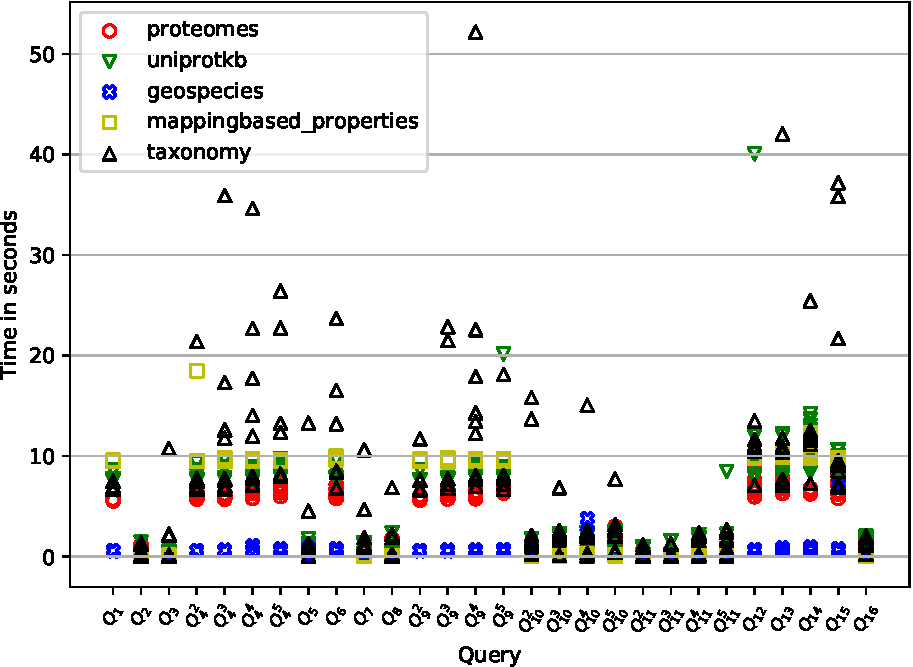
\includegraphics[width=0.48\textwidth]{data/other_all.pdf}
   \caption{Reachability index creation time for real-world RDFs}
   \label{fig:other_all_qs}
\end{figure}

Paths extraction was evaluated on cases with possible long paths.
These cases were selected during reachability index creation by using number of iterations in transitive closure evaluation.
For each selected graph and query we measure paths extraction time for each reachable pair, reachability index creation time is not included because exactly the same index, as calculated at the previous step, is used for paths extraction. 

We evaluate two scenarios.
The first one is a single path extraction.
In this case results are represented as a dependency of extraction time on extracted path length.
We can see linear !!!!

The second scenario is many paths extraction.
Here we limit a number of path to extract by !!! 
In this case results are represented as a dependency of extraction time on number of extracted paths.


\begin{figure}
     \begin{subfigure}[b]{0.24\textwidth}
         \centering
         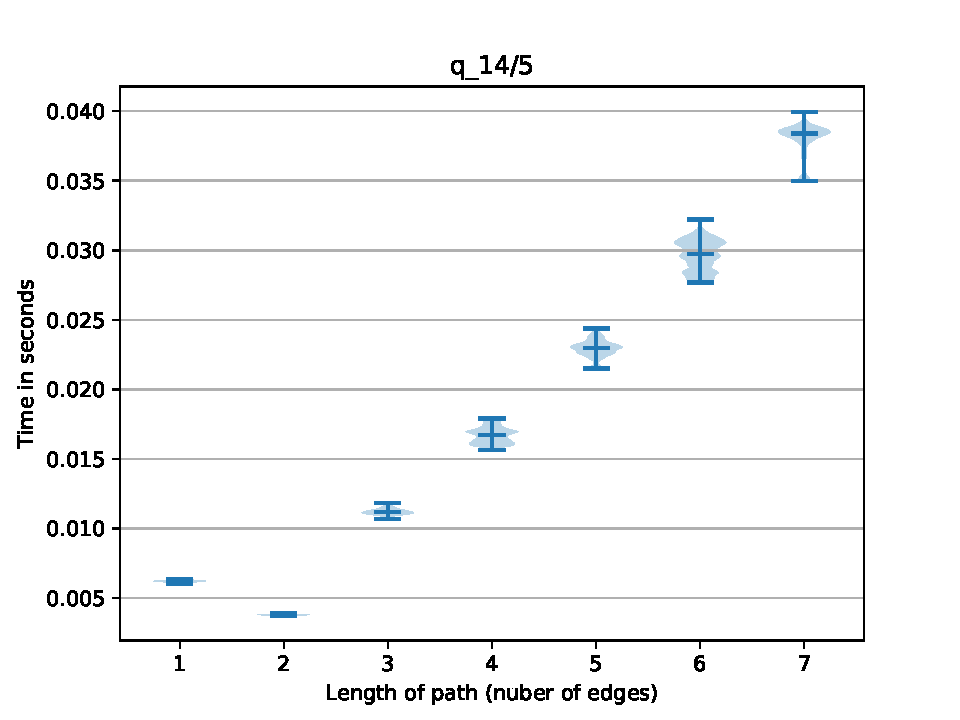
\includegraphics[width=\textwidth]{data/res_graphics/q_14_5.pdf}
         \caption{$y=x$}
         \label{fig:y equals x}
     \end{subfigure}
     ~\begin{subfigure}[b]{0.24\textwidth}
         \centering
         %\includegraphics[width=\textwidth]{data/res_graphics/q9_2_8.pdf}
         \caption{$y=x$}
         \label{fig:y equals x}
     \end{subfigure}\\
     \begin{subfigure}[b]{0.24\textwidth}
         \centering
         %\includegraphics[width=\textwidth]{data/res_graphics/q_14_8.pdf}
         \caption{$y=x$}
         \label{fig:y equals x}
     \end{subfigure}
     ~\begin{subfigure}[b]{0.24\textwidth}
         \centering
         %\includegraphics[width=\textwidth]{data/res_graphics/q4_2_8.pdf}
         \caption{$y=x$}
         \label{fig:y equals x}
     \end{subfigure}
   %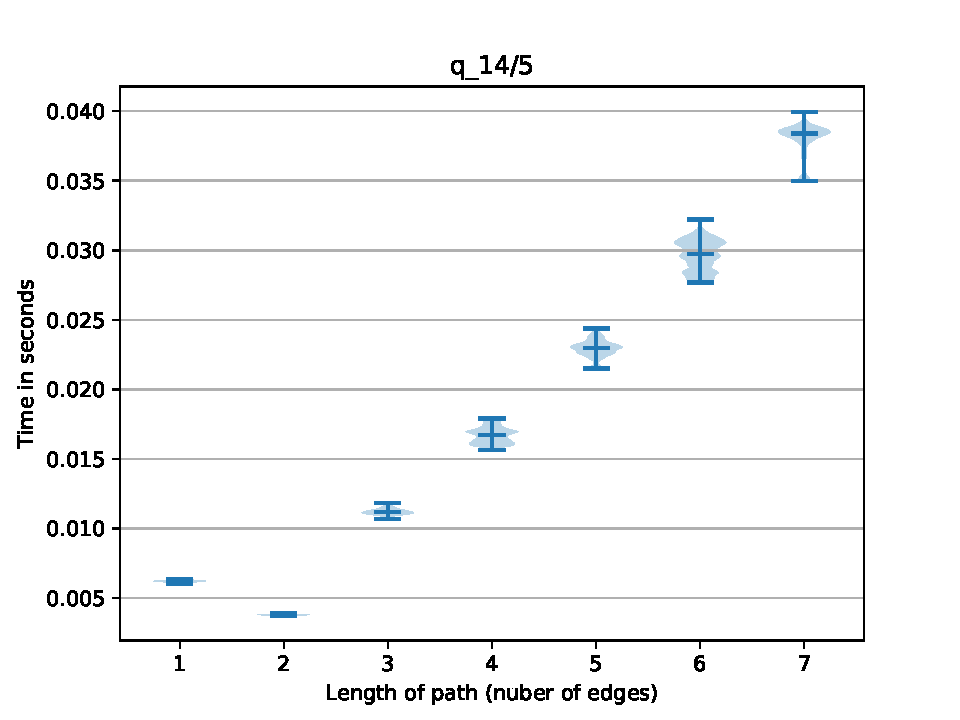
\includegraphics[width=0.48\textwidth]{data/res_graphics/q_14_5.pdf}
   \caption{Single path extraction}
\end{figure}

\subsubsection{Conclusion}

We can conclude that proposed algorithm is applicable for real-world data processing: the algorithm allows one both to solve reachability problem and to extract paths of interest in reasonable time even using na{\"i}ve implementation.  

\subsection{CFPQ Evaluation}

Comparison with matrix-based algorithm.

\subsubsection{Dataset}

Dataset for evaluation. 
It should be CFPQ\_Data\footnote{CFPQ\_Data is a dataset for CFPQ evaluation which contains both synthetic and real-world data and queries \url{https://github.com/JetBrains-Research/CFPQ\_Data}. Access date: 07.07.2020.}

\begin{table}
{
\rowcolors{2}{black!2}{black!10}
\begin{tabular}{|l|c|c|}
\hline
Graph & \#V & \#E \\
\hline
\hline 
eclass\_514en  & 120 926 & 484 646 \\
enzyme  & 358 434 & 144 9711 \\
geospecies  & 596 760 & 2 416 513 \\
go   & 1 188 340 & 4 820 728 \\
go-hierarchy & 1 780 956 & 7 228 358 \\
taxonomy & 2 308 385 & 9 369 511 \\
\hline
Aliases 1 & 6 442 630 & 24 465 430 \\
Aliases 2 & 4 834 262 & 12 366 973 \\
.... & 5 728 398 & 14 922 125 \\
\hline
\end{tabular}
}
\caption{Graphs for CFPQ evaluation}
\label{tbl:graphs_for_cfpq}
\end{table}



Same-generation queries, memory aliases.

\subsubsection{Results}

Results of evaluation.

Index creation.

{\setlength{\tabcolsep}{0.4em}
	\begin{table}
		\caption{RDFs query $G_1$ and $G_2$ (time is measured in seconds and memory is measured in megabytes)}
		\label{tbl:tableRDFQ1_appendix}
		\rowcolors{4}{black!2}{black!10}
		\small
		\begin{tabular}{| l | c | c | c | c |}
			\hline
			
			\multirow{2}{*}{Name}  & \multicolumn{2}{c|}{$G_1$} & \multicolumn{2}{c|}{$G_2$} \\
			\cline{2-5}
			                       & Tensors & RG\_CPU\textsubscript{path} & Tensors & RG\_CPU\textsubscript{path}	 \\
			\hline
			\hline
			eclass\_514en   & 0.254   & 0.195   & 0.227 & ...\\
			enzyme          & 0.035   & 0.029   & 0.036 & ...\\
			geospecies      & 0.091   & ...     & 0.001 & ...\\
			go-hierarchy    & 0.186   & 0.976   & 0.293 & ...\\
			go              & 1.676   & 1.286   & 1.368 & ...\\
			pathways        & 0.015   & 0.021   & 0.009 & ...\\
			taxonomy        & 5.366   & .....   & 3.282 & ...\\
			\hline
		\end{tabular}
	\end{table}
}


Paths extraction.

\subsubsection{Conclusion}

\section{Conclusion and future work}
In this paper, we shown how the context-free path query evaluation w.r.t. the relational and the single-path query semantics can be reduced to the calculation of matrix transitive closure. Also, we provided a formal proof of the correctness of the proposed reduction. In addition, we introduced an algorithm for computing this transitive closure, which allows us to efficiently apply GPGPU computing techniques. Finally, we shown the practical applicability of the proposed algorithm by running different implementations of our algorithm on real-world data.

We can identify several open problems for further research. In this paper we have considered only two semantics of context-free path querying but there are other important semantics, such as all-path query semantics~\cite{hellingsPathQuerying} which requires to present all paths for all triples $(A,m,n)$. Context-free path querying implemented with algorithm~\cite{GLL} can answer the queries in all-path query semantics by constructing a parse forest. It is possible to construct a parse forest for a linear input by matrix multiplication~\cite{okhotin_cyk}. Whether it is possible to generalize this approach for a graph input is an open question.

In our algorithm, we calculate the matrix transitive closure naively, but there are algorithms for the transitive closure calculation, which are asymptotically more efficient. Therefore, the question is whether it is possible to apply these algorithms for the matrix transitive closure calculation to the problem of context-free path querying.

Also, there are Boolean grammars~\cite{okhotinBoolean}, which have more expressive power than context-free grammars. Boolean path querying is an undecidable problem~\cite{hellingsRelational} but our algorithm can be trivially generalized to work on boolean grammars because parsing with boolean grammars can be expressed by matrix multiplication~\cite{okhotin_cyk}. It is not clear what a result of our algorithm applied to Boolean grammars would look like. Our hypothesis is that it would produce the upper approximation of a solution.

From a practical point of view, matrix multiplication in the main loop of the proposed algorithm may be performed on different GPGPU independently. It can help to utilize the power of multi-GPU systems and increase the performance of context-free path querying.

There is an algorithm~\cite{apspGPU} for transitive closure calculation on directed graphs which generalized to handle graph sizes inherently larger then the DRAM memory available on the GPU. Therefore, the question is whether it is possible to apply this approach to the matrix transitive closure calculation in the problem of context-free path querying.
 
\setmonofont[Mapping=tex-text]{CMU Typewriter Text}
\bibliographystyle{ugost2008ls}
\bibliography{diploma.bib}
\end{document}
